\DocumentMetadata{pdfversion=1.7,pdfstandard=A-3a,lang=zh-CN}
\documentclass[12pt,fontset=windows]{ctexart}

\usepackage{geometry}
\usepackage{xcolor}
\usepackage{caption}
\usepackage{tikz}
\usepackage{float}
\usepackage{amsmath}
\usepackage{lua-ul}
\usepackage{unicode-math}
\usepackage{fancyhdr}
\usepackage{hyperref}

\hypersetup{allcolors=blue,colorlinks}

\usetikzlibrary{calc,decorations.pathmorphing}

\geometry{a4paper,hmargin=1cm,vmargin=2cm}

\pagestyle{fancy}
\fancyhf{}
\fancyfoot[C]{\thepage}
\renewcommand{\headrulewidth}{0pt}
\renewcommand{\footrulewidth}{0pt}

% \newcommand{\answerWord}[1]{{\kaishu\color{blue}\underline{#1}}}
% \newcommand{\answerPar}[1]{{\kaishu\color{blue}{#1}}}
\newcommand{\answerWord}[1]{{\kaishu\underline{\;#1\;}}}
\newcommand{\answerPar}[1]{{\kaishu{#1}}}
\newcounter{selection}
\setcounter{selection}{1}
\newcommand{\resetCounter}{\setcounter{selection}{1}}
\newcommand{\showCounter}{\Alph{selection}.\stepcounter{selection}}
\newcommand{\selectionsFOURxONE}[4]{{
	\showCounter #1
	\hfill
	\showCounter #2
	\hfill
	\showCounter #3
	\hfill
	\showCounter #4
}}
\newcommand{\selectionsONExFOUR}[4]{{
	\showCounter #1

	\showCounter #2

	\showCounter #3

	\showCounter #4
}}

\newcommand{\selectionsTWOxTWO}[4]{{
	\showCounter #1
	\hfill
	\showCounter #2

	\showCounter #3
	\hfill
	\showCounter #4
}}

\title{高等工程力学期末考试样题}
\author{石成玉}
\date{\today}

\begin{document}

\section{单项选择题}
\begin{enumerate}
	\item 弹性力学研究（\answerWord{A}）由于受外力作用、边界约束或温度改变等原因而发生的应力、形变和位移。

	\resetCounter\selectionsFOURxONE{弹性体}{刚体}{粘性体}{塑性体}

	\item 弹性力学平面问题的求解中，平面应力问题与平面应变问题的三类基本方程具有下列关系（\answerWord{B}）。

	\resetCounter\selectionsONExFOUR{平衡方程、几何方程、物理方程完全相同}{平衡方程、几何方程相同，物理方程不同}{平衡方程、物理方程相同，几何方程不同}{平衡方程、几何方程、物理方程完全不相同}

	\item 平面问题的几何方程表述的是（\answerWord{D}）之间的关系
	
	\resetCounter\selectionsTWOxTWO{应力与体力}{应力与面力}{应力与应变}{应变与位移}
	
	\item 要使函数$\Phi(x,y)=axy^5+bx^5y$能作为应力函数，$a$与$b$的关系是（\answerWord{C}）

	\resetCounter\selectionsFOURxONE{$a$和$b$可任意取值}{$a=b$}{$a=-b$}{$a=\frac{b}{2}$}

	\item 对于三结点三角形单元，每个单元有3个结点，每个结点有（\answerWord{B}）个结点位移分量
	
	\resetCounter\selectionsFOURxONE{1}{2}{3}{4}
\end{enumerate}

\section{填空题}

\begin{enumerate}
	\item 弹性力学边界条件可以分为\answerWord{位移}边界条件、\answerWord{应变}边界条件和\answerWord{混合}边界条件。
	
	\begin{minipage}{0.7\linewidth}
		\item 按应力求解平面问题时，应力分量应当满足\answerWord{平衡微分}方程和\answerWord{相容}方程。此外，应力分量在边界上还应满足\answerWord{应力边界条件}。
		\item 杆件在竖直方向受到体力分量$f_y=f（常量）$的作用，其应力分量为：$\sigma_x=C_1 x$；$\sigma_y=C_2 y+C_3$；$\tau_xy=0$，支承条件如图\ref{pic:1}所示。则$C_1=$\answerWord{$0$}；$C_2=$\answerWord{$0$}；$C_3=$\answerWord{$f$}。
		\item 对平面应变问题，只需将平面应力问题的物理方程中材料常数作替换即可，即$E\rightarrow$\answerWord{$\frac{E}{1-\mu^2}$}；$\mu\rightarrow$\answerWord{$\frac{1}{1-\mu^2}$}。
	\end{minipage}
	\hfill
	\begin{minipage}{0.3\linewidth}
		\centering
		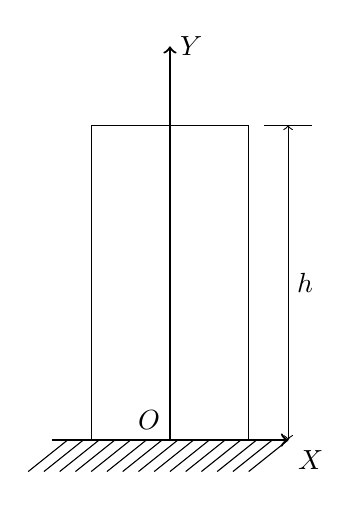
\begin{tikzpicture}
			\draw[thick,->] (0,0) -- (3,0) node[below right]{$X$};
			\draw[thick,->] (1.5,0) node[above left]{$O$} -- (1.5,5) node[right]{$Y$};
			\draw (0.5,0) rectangle (2.5,4);
			\draw (2.7,4) -- (3.3,4);
			\draw[<->] (3,4) -- node[right]{$h$} (3,0);
			\foreach \x in {0.2,0.4,...,3}{
				\draw (\x,0) -- ({\x-0.5},-0.4);
			}
		\end{tikzpicture}
		\captionof{figure}{}
		\label{pic:1}
	\end{minipage}
\end{enumerate}

%\begin{figure}[H]
%	\centering
%	\begin{tikzpicture}
%		\draw[thick,->] (0,0) -- (3,0) node[below right]{$X$};
%		\draw[thick,->] (1.5,0) node[above left]{$O$} -- (1.5,5) node[right]{$Y$};
%		\draw (0.5,0) rectangle (2.5,4);
%		\draw (2.7,4) -- (3.3,4);
%		\draw[<->] (3,4) -- node[right]{$h$} (3,0);
%		\foreach \x in {0.2,0.4,...,3}{
%			\draw (\x,0) -- ({\x-0.5},-0.4);
%		}
%	\end{tikzpicture}
%	\caption{}
%	\label{pic:1}
%\end{figure}

\section{简答题}

\begin{enumerate}
	\item 简述平面应力问题的基本特征并举例说明。

	\answerPar{特征：平面应力问题，就是只有平面应力分量（$\sigma_x$、$\sigma_y$和$\tau_{xy}$）存在，且仅为$x$，$y$的函数的弹性力学问题。}

	\answerPar{例子：设有很薄的等厚度薄板，只在板边上受有平行于板面并且不沿厚度变化的面力或约束（在板面上没有受到任何面力和约束）。同时体力也平行于板面并且不沿厚度变化。例如深梁，以及平板坝的平板支墩就属于此类问题。}

	\item 图示水坝（楔形体），试写出其应力边界条件。


	\begin{minipage}{0.3\linewidth}
		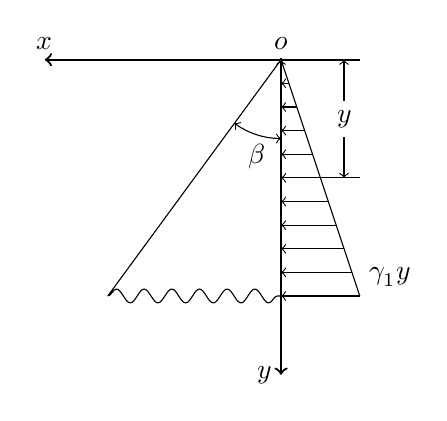
\begin{tikzpicture}
			\draw[thick,->] (1,0) -- (-3,0) node[above]{$x$};
			\draw[thick,->] (0,0) node[above]{$o$} -- (0,-4) node[left]{$y$};
			\draw[decoration={snake}] (0,0) -- (-2.2,-3) decorate{(-2.2,-3) -- (0,-3)};
			\draw[<->] (0,-1) arc (270:{180+atan(3/2.2)}:1) node[midway,below]{$\beta$};
			\foreach \t in {0,1,...,10}{
				\draw[->] ({0.1*\t},{-0.3*\t}) -- (0,{-0.3*\t});
			}
			\draw (0,0) -- ({0.1*10},{-0.3*10}) node[above right]{$\gamma_1 y$};
			\draw ({0.1*5},{-0.3*5}) -- ({0.1*10},{-0.3*5});
			\draw[<->] ({0.1*8},0) -- ({0.1*8},{-0.3*5}) node[midway,fill=white]{$y$};
		\end{tikzpicture}
	\end{minipage}
	\hfill
	\begin{minipage}{0.7\linewidth}
		$l$为单位长度面法线与$x$轴的投影，$m$为单位长度面法线与$y$轴的投影。

		$f_x$和$f_y$的正负同坐标轴方向。

		$\sigma_x$、$\sigma_y$：向外为正，向内为负。

		$\tau_{xy}$：以坐标轴方向为参考正负为$(\sigma_x \; \mathrm{or} \; \sigma_y)\times\tau_{xy}$。
	\end{minipage}

	\answerPar{
	\begin{minipage}{0.5\linewidth}
		左边界：
		\begin{gather*}
			l=\cos \beta, m=-\sin \beta \\
			\begin{cases}
				l\sigma_x + m\tau_{xy}=f_x=\cos \beta \sigma_x -\sin \beta \tau_{xy} = 0 \\
				m\sigma_y + l\tau_{xy} = -\sin\beta\sigma_y + \cos \beta \tau_{xy} = 0
			\end{cases}
		\end{gather*}
	\end{minipage}
	\begin{minipage}{0.5\linewidth}
		右边界：
		\begin{gather*}
			l=-1,m=0 \\
			\begin{cases}
				l\sigma_x + m\tau_{xy}=f_x=\sigma_x=\gamma_1 y \\
				m\sigma_y + l\tau_{xy} =\tau_{xy} = 0
			\end{cases}
		\end{gather*}
	\end{minipage}
	}

	\item 以三节点三角形单元为例，说明有限元分析法对离散结构的每个单元进行单元分析的具体内容和步骤。
	\item 边长为$1$的正方边形板结构分为\uppercase\expandafter{\romannumeral1}，\uppercase\expandafter{\romannumeral2}两个单元，单元编号、结点整体编码及各个单元局部编码如图所示，设通过单元分析已经得到这两个单元的刚度矩阵分别为$K^{(1)}$、$K^{(2)}$（即：单元刚度矩阵元素已知，其分块子矩阵可用符号表示）。试求这两个单元的刚度贡献矩阵$[K]^{(1)}$、$[K]^{(2)}$及离散系统的整体刚度矩阵$[K]$。
	
	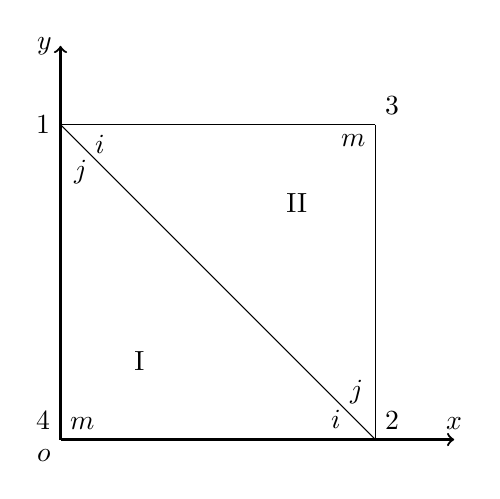
\begin{tikzpicture}
		\coordinate (O) at (0,0);
		\coordinate (Y) at (0,5);
		\coordinate (X) at (5,0);
		\coordinate (P1) at (0,4);
		\coordinate (P2) at (4,0);
		\coordinate (P3) at (4,4);
		\draw[->,thick] (O) -- (Y);
		\draw[->,thick] (O) -- (X);
		\draw (P1) -- (P3);
		\draw (P3) -- (P2);
		\draw (P1) -- (P2);
		\node[below left] at (O) {$o$};
		\node[above right] at (O) {$m$};
		\node[left] at (Y) {$y$};
		\node[above] at (X) {$x$};
		\node[above left] at (O) {$4$};
		\node[left] at (P1) {$1$};
		\node[above right] at (P2) {$2$};
		\node[above right] at (P3) {$3$};
		\node[below left] at (P3) {$m$};
		\node at ($(P1) + (0.5,-0.25)$) {$i$};
		\node at ($(P1) + (0.25,-0.6)$) {$j$};
		\node at ($(P2) + (-0.25,0.6)$) {$j$};
		\node at ($(P2) + (-0.5,0.25)$) {$i$};
		\node at (1,1) {\uppercase\expandafter{\romannumeral1}};
		\node at (3,3) {\uppercase\expandafter{\romannumeral2}};
	\end{tikzpicture}
\end{enumerate}

\section{分析计算题}

\begin{enumerate}
	\item 图所示的悬臂梁，长度为$l$，高度为$h$，$l>>h$，在上边界受匀布荷载$q$，试检验应力函数$\varPhi=Ay^5+Bx^2y^3+Cy^3+Dx^2+Ex^2y$能否成为此问题的解？如可以，试求出应力分量。
	
	\begin{minipage}{0.4\linewidth}
		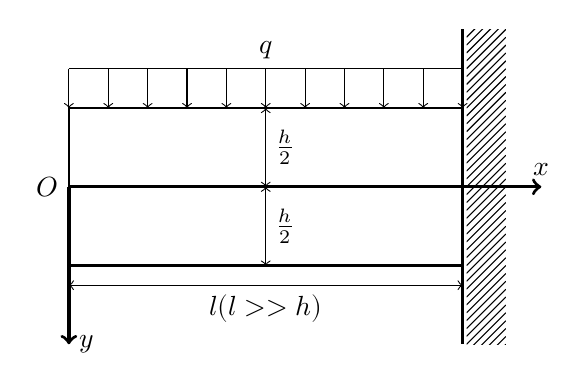
\begin{tikzpicture}
			\draw[very thick,->] (0,0) node[left]{$O$} -- (6,0) node[above]{$x$};
			\draw[very thick,->] (0,0) -- (0,-2) node[right]{$y$};
			\draw[thick] (0,1) rectangle (5,-1);
			\foreach \x in {0,0.5,...,5}{
				\draw[->] (\x,1.5) -- (\x,1);
			}
			\draw[<->] (2.5,0) -- (2.5,1) node[midway,right]{$\frac{h}{2}$};
			\draw[<->] (2.5,0) -- (2.5,-1)node[midway,right]{$\frac{h}{2}$};
			\draw[<->] (0,-1.25) -- (5,-1.25) node[midway,below]{$l(l>>h)$};
			\draw[very thick] (5,2) -- (5,-2);
			\begin{scope}
				\clip (5.05,2) rectangle (5.55,-2);
				\foreach \y in {-3,-2.9,...,2}{
					\draw (5.05,\y) -- ++(0.5,0.5);
				}
			\end{scope}
			\draw (0,1.5) -- (5,1.5) node[midway,above]{$q$};
		\end{tikzpicture}
	\end{minipage}
	\hfill
	\begin{minipage}{0.6\linewidth}
		应力函数$\varPhi$需满足应力函数表示的相容方程：
		\begin{equation}
			\frac{\partial^4\varPhi}{\partial x^4}+2\frac{\partial^4 \varPhi}{\partial x^2 \partial y^2}+\frac{\partial^4 \varPhi}{\partial y^4}=0 \label{eq:应力函数表示的相容方程}
		\end{equation}
		再满足边界条件，求得待定系数后代入平衡微分方程全解求应力分量：
		\begin{equation}
			\sigma_x = \frac{\partial^2 \varPhi}{\partial y^2}-f_x x,\sigma_y=\frac{\partial^2 \varPhi}{\partial x^2}-f_y y,\tau_{xy}=-\frac{\partial^2 \varPhi}{\partial x \partial y}\label{eq:平衡微分方程全解}
		\end{equation}
	\end{minipage}

	\answerPar{2阶4阶偏导：}

	\begin{minipage}{0.5\linewidth}
		\begin{align*}
			\frac{\partial^2\varPhi}{\partial x^2}&=2By^3+2D+2Ey \\
			\frac{\partial^2\varPhi}{\partial y^2}&=20Ay^3+6Bx^2y+6Cy \\
			\frac{\partial^2 \varPhi}{\partial x\partial y}&=6Bxy^2+2Ex
		\end{align*}
	\end{minipage}
	\begin{minipage}{0.5\linewidth}
		\begin{align*}
			\frac{\partial^4\varPhi}{\partial x^4}&=0 \\
			\frac{\partial^4 \varPhi}{\partial x^4}&=120Ay \\
			\frac{\partial^4 \varPhi}{\partial x^2 \partial y^2}&=12By
		\end{align*}
	\end{minipage}

	\answerPar{边界条件：}

	\begin{minipage}{0.5\linewidth}
		\answerPar{上边界：}$y=-\frac{h}{2}$
		\begin{gather*}
			l=0,m=-1 \\
			-\tau_{xy}=0 \\
			-\sigma_y=q
		\end{gather*}
	\end{minipage}
	\hfill
	\begin{minipage}{0.5\linewidth}
		\answerPar{下边界：}$y=\frac{h}{2}$
		\begin{gather*}
			l=0,m=1 \\
			\tau_{xy}=0 \\
			\sigma_y=0
		\end{gather*}
	\end{minipage}

	\answerPar{代入公式\eqref{eq:应力函数表示的相容方程}：}

	\begin{gather*}
		0+24By+120Ay=0 \rightarrow B+5A=0 \rightarrow B=-5A
	\end{gather*}

	\answerPar{代入公式\eqref{eq:平衡微分方程全解}：}

	\begin{align*}
		-6Bx(-\frac{h}{2})^2-2Ex=0 & \rightarrow E=-\frac{3}{4}Bh^2 \\
		2B(-\frac{h}{2})^3+2D+2E(-\frac{h}{2})=-q & \rightarrow -\frac{1}{4}Bh^3+2D-Eh=-q \\
		2B(\frac{h}{2})^3+2D+2E\frac{h}{2}=0 & \rightarrow \frac{1}{4}Bh^3+2D+Eh=0
	\end{align*}

	\answerPar{4个等式对应4个未知量，求解得：}

	\begin{equation*}
		A=\frac{q}{5h^3}, \quad B=-\frac{q}{h^3}, \quad D=-\frac{q}{4}, \quad E= \frac{3q}{4h}
	\end{equation*}

	\answerPar{该应力函数能成为此问题的解。应力分量：}

	\begin{align*}
		\sigma_x&=\frac{4q}{h^3}y^3-\frac{6q}{h^3}x^2y+6Cy \\
		\sigma_y&=-\frac{2q}{h^3}y^3-\frac{q}{2}+\frac{3q}{2h}y \\
		\tau_{xy}&=-\frac{6q}{h^3}xy^2+\frac{3q}{2h}x
	\end{align*}

	\item 如图所示的矩形截面柱体，在顶部受有集中力$\boldsymbol{F}$和力矩$\boldsymbol{M}=\frac{Fb}{2}$的作用，试用应力函数$\varPhi=Ax^3+Bx^2$求解图示问题的应力及位移，设在$A$点的位移和转角均为零。
	
	\begin{minipage}{0.4\linewidth}
		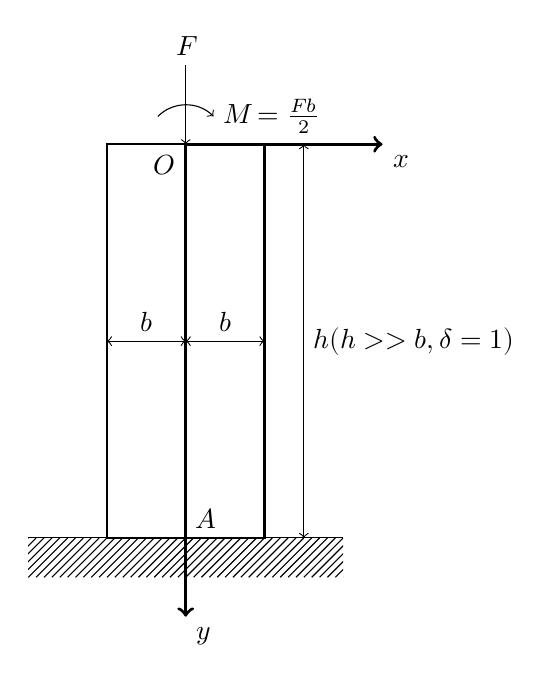
\begin{tikzpicture}
			\draw[very thick,->] (0,0) node[below left]{$O$}-- (2.5,0) node[below right]{$x$};
			\draw[very thick,->] (0,0) -- (0,-6) node[below right]{$y$};
			\draw[thick] (-1,0) rectangle (1,-5);
			\draw (-2,-5) -- (2,-5);
			\begin{scope}
				\clip (-2,-5) rectangle (2,-5.5);
				\foreach \x in {-2,-1.9,...,3}{
					\draw (\x,-5) -- ++(-0.5,-0.5);
				}
			\end{scope}
			\draw[<->] (1.5,0) -- (1.5,-5) node[midway,right]{$h(h>>b,\delta=1)$};
			\draw[<->] (-1,-2.5) -- (0,-2.5) node[midway,above]{$b$};
			\draw[<->] (1,-2.5) -- (0,-2.5) node[midway,above]{$b$};
			\node[above right] at (0,-5) {$A$};
			\draw[->] (0,1) -- (0,0) node[pos=0,above]{$\boldsymbol{F}$};
			\draw[->] (135:0.5) arc (135:45:0.5) node[pos=1,right]{$\boldsymbol{M}=\frac{Fb}{2}$};
		\end{tikzpicture}
	\end{minipage}
	\hfill
	\begin{minipage}{0.6\linewidth}
		利用公式\eqref{eq:应力函数表示的相容方程}和\eqref{eq:平衡微分方程全解}求解出艾里应力函数中的常数。再根据平面问题的物理方程：
		\begin{equation}
			\left\{
				\begin{aligned}
					\varepsilon_x=\frac{1}{E}(\sigma_x-\mu\sigma_y) \\
					\varepsilon_y=\frac{1}{E}(\sigma_y-\mu\sigma_x) \\
					\gamma_{xy}=\frac{2(1+\mu)}{E}\tau_{xy}
				\end{aligned}
			\right.
			\label{eq:平面问题的物理方程}
		\end{equation}
		和平面问题的几何方程：
		\begin{equation}
			\varepsilon_x=\frac{\partial u}{\partial x},\,\varepsilon=\frac{\partial v}{\partial y},\,\gamma=\frac{\partial v}{\partial x}+\frac{\partial u}{\partial y}
			\label{eq:平面问题的几何方程}
		\end{equation}
		求解位移。
	\end{minipage}

	\begin{minipage}[t]{0.5\linewidth}
		\answerPar{应力分量：}
		\begin{align*}
			\sigma_x&=\frac{\partial^2\varPhi}{\partial y^2}=0 \\
			\sigma_y&=\frac{\partial^2\varPhi}{\partial x^2}=6Ax+2B \\
			\tau_{yx}&=0
		\end{align*}
	\end{minipage}
	\hfill
	\begin{minipage}[t]{0.5\linewidth}
		\answerPar{边界条件：}
		\begin{gather*}
			y=0:\ l=0,\;m=-1 \\
			\int_{-b}^{b}-\tau_{yx}\mathrm{d}x=0 \\
			\int_{-b}^{b}-\sigma_y\mathrm{d}x=\boldsymbol{F} \\
			\int_{-b}^{b}-\sigma_y y\mathrm{d}x=\frac{\boldsymbol{Fb}}{2} \\
		\end{gather*}
	\end{minipage}

	\answerPar{代入得：}
	\begin{equation*}
		\begin{cases}
			\int_{-b}^{b}6Ax+2B\mathrm{d}x=-\boldsymbol{F} \\
			\int_{-b}^{b}6Ax^2+2Bx\mathrm{d}x=-\frac{\boldsymbol{Fb}}{2}
		\end{cases}
		\Longrightarrow
		\begin{cases}
			A=-\frac{F}{8b^2} \\
			B=-\frac{F}{4b}
		\end{cases}
	\end{equation*}
	\answerPar{故：}
	\begin{equation*}
%		\color{blue}
		\sigma_y=-\frac{3F}{4b^2}x-\frac{F}{2b}
	\end{equation*}
	\answerPar{代入公式\eqref{eq:平面问题的几何方程}：}
	\begin{equation*}
		\varepsilon_y=\frac{1}{E}\sigma_y=\frac{\partial u}{\partial y} \Longrightarrow u=\frac{1}{E}\sigma_yy+C(x)
	\end{equation*}
	\answerPar{根据题目$A$点的位移和转角均为零，代入$y=h$、$u=0$、$\omega=0$：}
	\begin{equation*}
		C(x)=-\frac{1}{E}\sigma_yh \Longrightarrow u=\frac{1}{E}\sigma_y(y-h)
	\end{equation*}
	\answerPar{故：}
	\begin{equation*}
%		\color{blue}
		u=\frac{1}{E}\left(\frac{3F}{4b^2}+\frac{F}{2b}\right)(h-y)
	\end{equation*}

\end{enumerate}

\end{document}